This chapter evaluates and discusses how successful the design and implementation was at meeting the proposed requirements for the project. To do this, the chapter will discuss how the protocol was tested to satisfy the initial use cases, the implementation size, followed by a comparison of the efficiency of the protocol and its implementation to the eXtensible Application protocol (xAP) discussed in chapter \ref{cha:background}.


\section{Testing} % (fold)
\label{sec:testing}
To ensure the protocol worked throughout development, both the simulator and TelosB motes were used to test some of the scenarios described in the use cases contained in chapter \ref{cha:requirements_gathering}.
\subsection{Sensor logging} % (fold)
\label{sub:sensor_logging}
In order to test the multiple channel support of devices, the scenario of sensor logging was set up; where one or more controllers search the network for available sensors and request data from them at regular intervals.
To demonstrate this, the scenario was set up in the Cooja simulator, with one controller device, three light sensor devices and three actuators; the controller was set to locate and connect to three sensing devices which could sense light.

In figure \ref{fig:logtest}, the controller is labelled as mote 1, and can be seen to receive messages from sensor motes 3, 5, 7. Motes 8, 9, 10 are actuators motes, listening for any broadcast queries which match their type. In the mote output box, each mote prints out its temperature locally, as designated by the Mote column, and sends it to the controller, where it also prints it.

\begin{figure}[h]
\centering
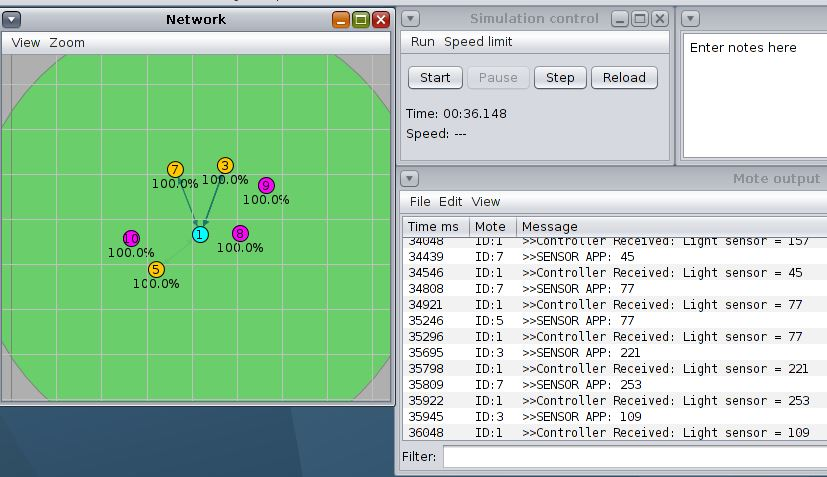
\includegraphics[scale=0.5]{evaluation/img/logTest.jpg}
\caption{Sensor logging scenario}
\label{fig:logtest}
\end{figure}  
% subsection sensor_logging (end)

\subsection{Light/Presence detector} % (fold)
\label{sub:presence_detector}
In order to ensure multiple types of devices could be connected, so that a closed loop system could be created, a scenario involving a controller, light sensor and light switch was created. The controller attempts to locate and connect to a light sensor and light switch actuator on the network, using the readings from the light sensor to decide when to turn the light switch on and off. The purpose of such a scenario is to demonstrate the possibility of the ``Internet of Things'' sensing either, the presence of a user by obscuring a sensor, or the change in lighting conditions, which would require a light to be turned on to assist the user.
To test and demonstrate this, the scenario was set up using both real motes and the simulator, with one controller device, one light sensor device and one light switch actuator device.

In figure \ref{fig:lighttest}, the controller is labelled as mote 2, and can be seen to receive messages from sensor mote 1 and send messages to actuator mote 3. In the Mote output box, the various print outs can be seen, displaying sensor readings received, decisions based on the sensor readings and the commands sent and received. In the network view box, it's possible to see the LEDs on mote 3 alight, due to the recent command to turn on the lights.

\begin{figure}[h]
\centering
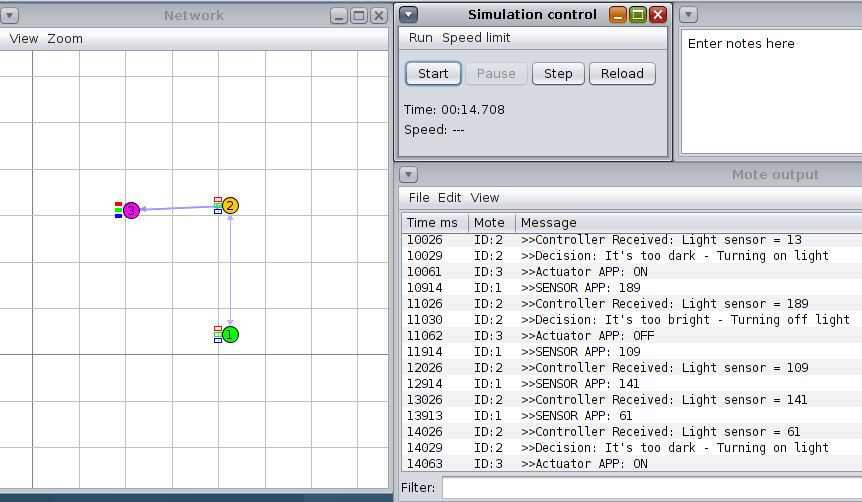
\includegraphics[scale=0.5]{evaluation/img/lightswitch.jpg}
\caption{Light/Presence detector}
\label{fig:lighttest}
\end{figure}

% subsection presence_detector (end)
% section testing (end)

\section{Implementation size} % (fold)
\label{sec:implementation_size_and_performance}
Creating a lightweight protocol is one of the primary requirements, thus ensuring that the protocol could be implemented on even the most constrained devices, such as the TelosB or Arduino. Because of this, each aspect in the protocol had to be made as low cost as possible, whilst still maintaining flexibility and upgradeability. With this in mind the TelosB implementation performs well in regards to consuming device resources, as show in figure \cite{size} when compared to a variety of other application.

To demonstrate the amount of ROM and RAM occupied, a simple hello world program was created, which upon receiving an event, output ``Hello world'' to serial. This provided the baseline from which to compare the implementation against; also included as another baseline is the same hello world program with uIP included, which shows how much is added to the binary without any additional code being written.

When comparing the Hello world app with the Hello world app with uIP included, a significant difference can be seen in the size of ROM consumed as well the RAM, leaving around 18,000 bytes ROM and around 3,300 bytes RAM left for an application and other libraries.

Comparing the sensor implementation of the IoT protocol with uIP and a minimal sensor application to connect a sensor to the API and print out a message, consumes only an additional 2428 bytes ROM and 994 bytes RAM with 10 channels and 554 bytes RAM with 5 channels.
Similarly the actuator implementation performs on par, only consuming a minimal amount more in both cases. Unlike the two other implementations, the controller implementation consumes a much higher, 3848 bytes of ROM but a minimal increase in RAM, due to the necessity to discover, communicate and connect to both of the other device roles.
\begin{figure}[h]
\begin{center}
    \begin{tabular}{| l | c | c | c | l |}
    \hline
    Setup & ROM (bytes) & RAM (bytes) & Channels & Notes \\ \hline
    Hello world & 19,812 & 5,538 & n/a &... \\ \hline
    Hello world & 29,494 & 6,764 & n/a & with uIP stack. \\ \hline
    Sensor app & 31,922 & 7,708 & 10 & with uIP stack, IoT Protocol and light sensor\\ \hline
    Actuator app & 32,032 & 7,750 & 10 & with uIP stack, IoT Protocol and LEDs \\ \hline
    Controller app & 33,318 & 7,808 & 10 & with uIP stack, IoT Protocol \\ \hline
    Sensor app & 31,922 & 7,318 & 5 & with uIP stack, IoT Protocol and light sensor\\ \hline
    Actuator app & 32,032 & 7,320 & 5 & with uIP stack, IoT Protocol and LEDs \\ \hline
    Controller app & 33,318 & 7,378 & 5 & with uIP stack, IoT Protocol \\ 
    \hline
    \end{tabular}
\end{center}
\caption{Table showing implementation sizes against stock Contiki}
\label{tab:size}
\end{figure}



Discuss size of protocol implementation and general performance.

currently frequencies limited to ints not floats, but could be upgraded to support finer time intervals without any problems.
% section implementation_size_and_performance (end)

\section{Comparison to other systems} % (fold)
\label{sec:comparison_to_other_systems}
To better demonstrate the lightweight nature of the protocol and also the scalability which it can provide, two scenarios are demonstrated in figures \ref{graph:IoT1}\ref{graph:IoT2}
\subsection{xAP - Receiving packets} % (fold)
\label{sub:xap}

calculate number of packets received by one node for both systems in a typical scenario, as the network expands to support 5, 10, 25 50, 100, 200 nodes.


\begin{figure}[h]
\begin{center}
\begin{minipage}{.5\textwidth}
\begin{tikzpicture}[gnuplot]
%% generated with GNUPLOT 4.7p0 (Lua 5.1; terminal rev. 99, script rev. 100)
%% Wed 15 May 2013 18:37:35 BST
\gpsolidlines
\path (0.000,0.000) rectangle (12.500,8.750);
\gpcolor{color=gp lt color border}
\gpsetlinetype{gp lt border}
\gpsetlinewidth{1.00}
\draw[gp path] (1.504,0.985)--(1.684,0.985);
\node[gp node right] at (1.320,0.985) { 0};
\draw[gp path] (1.504,1.281)--(1.594,1.281);
\draw[gp path] (1.504,1.577)--(1.684,1.577);
\node[gp node right] at (1.320,1.577) { 20};
\draw[gp path] (1.504,1.873)--(1.594,1.873);
\draw[gp path] (1.504,2.168)--(1.684,2.168);
\node[gp node right] at (1.320,2.168) { 40};
\draw[gp path] (1.504,2.464)--(1.594,2.464);
\draw[gp path] (1.504,2.760)--(1.684,2.760);
\node[gp node right] at (1.320,2.760) { 60};
\draw[gp path] (1.504,3.056)--(1.594,3.056);
\draw[gp path] (1.504,3.352)--(1.684,3.352);
\node[gp node right] at (1.320,3.352) { 80};
\draw[gp path] (1.504,3.648)--(1.594,3.648);
\draw[gp path] (1.504,3.943)--(1.684,3.943);
\node[gp node right] at (1.320,3.943) { 100};
\draw[gp path] (1.504,4.239)--(1.594,4.239);
\draw[gp path] (1.504,4.535)--(1.684,4.535);
\node[gp node right] at (1.320,4.535) { 120};
\draw[gp path] (1.504,4.831)--(1.594,4.831);
\draw[gp path] (1.504,5.127)--(1.684,5.127);
\node[gp node right] at (1.320,5.127) { 140};
\draw[gp path] (1.504,5.423)--(1.594,5.423);
\draw[gp path] (1.504,5.718)--(1.684,5.718);
\node[gp node right] at (1.320,5.718) { 160};
\draw[gp path] (1.504,6.014)--(1.594,6.014);
\draw[gp path] (1.504,6.310)--(1.684,6.310);
\node[gp node right] at (1.320,6.310) { 180};
\draw[gp path] (1.504,6.606)--(1.594,6.606);
\draw[gp path] (1.504,6.902)--(1.684,6.902);
\node[gp node right] at (1.320,6.902) { 200};
\draw[gp path] (1.504,7.198)--(1.594,7.198);
\draw[gp path] (1.504,7.493)--(1.684,7.493);
\node[gp node right] at (1.320,7.493) { 220};
\draw[gp path] (1.504,7.789)--(1.594,7.789);
\draw[gp path] (1.504,8.085)--(1.684,8.085);
\node[gp node right] at (1.320,8.085) { 240};
\draw[gp path] (1.504,8.381)--(1.594,8.381);
\draw[gp path] (3.177,0.985)--(3.177,1.165);
\node[gp node center] at (3.177,0.677) {Controller};
\draw[gp path] (4.851,0.985)--(4.851,1.165);
\node[gp node center] at (4.851,0.677) {Actuator};
\draw[gp path] (6.524,0.985)--(6.524,1.165);
\node[gp node center] at (6.524,0.677) {Sensor};
\draw[gp path] (1.504,8.381)--(1.504,0.985)--(8.197,0.985)--(8.197,8.381)--cycle;
\node[gp node center,rotate=-270] at (0.246,4.683) {Total messages received};
\node[gp node center] at (4.850,0.215) {Device Type};
\node[gp node right] at (6.729,8.047) {Sense Msg};
\gpfill{color=gp lt color 0} (6.913,7.970)--(7.829,7.970)--(7.829,8.124)--(6.913,8.124)--cycle;
\gpsetlinetype{gp lt plot 0}
\draw[gp path] (6.913,7.970)--(7.829,7.970)--(7.829,8.124)--(6.913,8.124)--cycle;
\gpfill{color=gp lt color 0} (2.550,0.985)--(3.806,0.985)--(3.806,2.761)--(2.550,2.761)--cycle;
\draw[gp path] (2.550,0.985)--(2.550,2.760)--(3.805,2.760)--(3.805,0.985)--cycle;
\node[gp node right] at (6.729,7.739) {Command Msg};
\gpfill{color=gp lt color 1} (6.913,7.662)--(7.829,7.662)--(7.829,7.816)--(6.913,7.816)--cycle;
\gpsetlinetype{gp lt plot 1}
\draw[gp path] (6.913,7.662)--(7.829,7.662)--(7.829,7.816)--(6.913,7.816)--cycle;
\gpfill{color=gp lt color 1} (2.550,2.760)--(3.806,2.760)--(3.806,2.761)--(2.550,2.761)--cycle;
\draw[gp path] (2.550,2.760)--(3.805,2.760)--cycle;
\gpfill{color=gp lt color 1} (4.223,0.985)--(5.479,0.985)--(5.479,1.430)--(4.223,1.430)--cycle;
\draw[gp path] (4.223,0.985)--(4.223,1.429)--(5.478,1.429)--(5.478,0.985)--cycle;
\node[gp node right] at (6.729,7.431) {Sensor Ping};
\gpfill{color=gp lt color 2} (6.913,7.354)--(7.829,7.354)--(7.829,7.508)--(6.913,7.508)--cycle;
\gpsetlinetype{gp lt plot 2}
\draw[gp path] (6.913,7.354)--(7.829,7.354)--(7.829,7.508)--(6.913,7.508)--cycle;
\gpfill{color=gp lt color 2} (2.550,2.760)--(3.806,2.760)--(3.806,2.939)--(2.550,2.939)--cycle;
\draw[gp path] (2.550,2.760)--(2.550,2.938)--(3.805,2.938)--(3.805,2.760)--cycle;
\gpfill{color=gp lt color 2} (4.223,1.429)--(5.479,1.429)--(5.479,1.430)--(4.223,1.430)--cycle;
\draw[gp path] (4.223,1.429)--(5.478,1.429)--cycle;
\node[gp node right] at (6.729,7.123) {Actuator Ping};
\gpfill{color=gp lt color 3} (6.913,7.046)--(7.829,7.046)--(7.829,7.200)--(6.913,7.200)--cycle;
\gpsetlinetype{gp lt plot 3}
\draw[gp path] (6.913,7.046)--(7.829,7.046)--(7.829,7.200)--(6.913,7.200)--cycle;
\gpfill{color=gp lt color 3} (2.550,2.938)--(3.806,2.938)--(3.806,2.939)--(2.550,2.939)--cycle;
\draw[gp path] (2.550,2.938)--(3.805,2.938)--cycle;
\gpfill{color=gp lt color 3} (4.223,1.429)--(5.479,1.429)--(5.479,1.430)--(4.223,1.430)--cycle;
\draw[gp path] (4.223,1.429)--(5.478,1.429)--cycle;
\node[gp node right] at (6.729,6.815) {ACK};
\gpfill{color=gp lt color 4} (6.913,6.738)--(7.829,6.738)--(7.829,6.892)--(6.913,6.892)--cycle;
\gpsetlinetype{gp lt plot 4}
\draw[gp path] (6.913,6.738)--(7.829,6.738)--(7.829,6.892)--(6.913,6.892)--cycle;
\gpfill{color=gp lt color 4} (2.550,2.938)--(3.806,2.938)--(3.806,3.382)--(2.550,3.382)--cycle;
\draw[gp path] (2.550,2.938)--(2.550,3.381)--(3.805,3.381)--(3.805,2.938)--cycle;
\gpfill{color=gp lt color 4} (4.223,1.429)--(5.479,1.429)--(5.479,1.430)--(4.223,1.430)--cycle;
\draw[gp path] (4.223,1.429)--(5.478,1.429)--cycle;
\gpfill{color=gp lt color 4} (5.896,0.985)--(7.152,0.985)--(7.152,1.164)--(5.896,1.164)--cycle;
\draw[gp path] (5.896,0.985)--(5.896,1.163)--(7.151,1.163)--(7.151,0.985)--cycle;
\gpsetlinetype{gp lt border}
\draw[gp path] (1.504,8.381)--(1.504,0.985)--(8.197,0.985)--(8.197,8.381)--cycle;
%% coordinates of the plot area
\gpdefrectangularnode{gp plot 1}{\pgfpoint{1.504cm}{0.985cm}}{\pgfpoint{8.197cm}{8.381cm}}
\end{tikzpicture}
%% gnuplot variables

\caption{Packets received in 1 minute using IoT protocol}
\label{graph:IoT1}
\end{minipage}%
\begin{minipage}{.5\textwidth}
\begin{tikzpicture}[gnuplot]
%% generated with GNUPLOT 4.7p0 (Lua 5.1; terminal rev. 99, script rev. 100)
%% Fri 26 Apr 2013 15:19:36 BST
\gpsolidlines
\path (0.000,0.000) rectangle (12.500,8.750);
\gpcolor{color=gp lt color border}
\gpsetlinetype{gp lt border}
\gpsetlinewidth{1.00}
\draw[gp path] (1.504,0.985)--(1.684,0.985);
\node[gp node right] at (1.320,0.985) { 0};
\draw[gp path] (1.504,1.281)--(1.594,1.281);
\draw[gp path] (1.504,1.577)--(1.684,1.577);
\node[gp node right] at (1.320,1.577) { 20};
\draw[gp path] (1.504,1.873)--(1.594,1.873);
\draw[gp path] (1.504,2.168)--(1.684,2.168);
\node[gp node right] at (1.320,2.168) { 40};
\draw[gp path] (1.504,2.464)--(1.594,2.464);
\draw[gp path] (1.504,2.760)--(1.684,2.760);
\node[gp node right] at (1.320,2.760) { 60};
\draw[gp path] (1.504,3.056)--(1.594,3.056);
\draw[gp path] (1.504,3.352)--(1.684,3.352);
\node[gp node right] at (1.320,3.352) { 80};
\draw[gp path] (1.504,3.648)--(1.594,3.648);
\draw[gp path] (1.504,3.943)--(1.684,3.943);
\node[gp node right] at (1.320,3.943) { 100};
\draw[gp path] (1.504,4.239)--(1.594,4.239);
\draw[gp path] (1.504,4.535)--(1.684,4.535);
\node[gp node right] at (1.320,4.535) { 120};
\draw[gp path] (1.504,4.831)--(1.594,4.831);
\draw[gp path] (1.504,5.127)--(1.684,5.127);
\node[gp node right] at (1.320,5.127) { 140};
\draw[gp path] (1.504,5.423)--(1.594,5.423);
\draw[gp path] (1.504,5.718)--(1.684,5.718);
\node[gp node right] at (1.320,5.718) { 160};
\draw[gp path] (1.504,6.014)--(1.594,6.014);
\draw[gp path] (1.504,6.310)--(1.684,6.310);
\node[gp node right] at (1.320,6.310) { 180};
\draw[gp path] (1.504,6.606)--(1.594,6.606);
\draw[gp path] (1.504,6.902)--(1.684,6.902);
\node[gp node right] at (1.320,6.902) { 200};
\draw[gp path] (1.504,7.198)--(1.594,7.198);
\draw[gp path] (1.504,7.493)--(1.684,7.493);
\node[gp node right] at (1.320,7.493) { 220};
\draw[gp path] (1.504,7.789)--(1.594,7.789);
\draw[gp path] (1.504,8.085)--(1.684,8.085);
\node[gp node right] at (1.320,8.085) { 240};
\draw[gp path] (1.504,8.381)--(1.594,8.381);
\draw[gp path] (3.177,0.985)--(3.177,1.165);
\node[gp node center] at (3.177,0.677) {Controller};
\draw[gp path] (4.851,0.985)--(4.851,1.165);
\node[gp node center] at (4.851,0.677) {Actuator};
\draw[gp path] (6.524,0.985)--(6.524,1.165);
\node[gp node center] at (6.524,0.677) {Sensor};
\draw[gp path] (1.504,8.381)--(1.504,0.985)--(8.197,0.985)--(8.197,8.381)--cycle;
\node[gp node center,rotate=-270] at (0.246,4.683) {Total messages received};
\node[gp node center] at (4.850,0.215) {Device Type};
\node[gp node right] at (6.729,8.047) {Sense Msg};
\gpfill{color=gp lt color 0} (6.913,7.970)--(7.829,7.970)--(7.829,8.124)--(6.913,8.124)--cycle;
\gpsetlinetype{gp lt plot 0}
\draw[gp path] (6.913,7.970)--(7.829,7.970)--(7.829,8.124)--(6.913,8.124)--cycle;
\gpfill{color=gp lt color 0} (2.550,0.985)--(3.806,0.985)--(3.806,2.761)--(2.550,2.761)--cycle;
\draw[gp path] (2.550,0.985)--(2.550,2.760)--(3.805,2.760)--(3.805,0.985)--cycle;
\gpfill{color=gp lt color 0} (4.223,0.985)--(5.479,0.985)--(5.479,2.761)--(4.223,2.761)--cycle;
\draw[gp path] (4.223,0.985)--(4.223,2.760)--(5.478,2.760)--(5.478,0.985)--cycle;
\node[gp node right] at (6.729,7.739) {Command Msg};
\gpfill{color=gp lt color 1} (6.913,7.662)--(7.829,7.662)--(7.829,7.816)--(6.913,7.816)--cycle;
\gpsetlinetype{gp lt plot 1}
\draw[gp path] (6.913,7.662)--(7.829,7.662)--(7.829,7.816)--(6.913,7.816)--cycle;
\gpfill{color=gp lt color 1} (2.550,2.760)--(3.806,2.760)--(3.806,2.761)--(2.550,2.761)--cycle;
\draw[gp path] (2.550,2.760)--(3.805,2.760)--cycle;
\gpfill{color=gp lt color 1} (4.223,2.760)--(5.479,2.760)--(5.479,3.205)--(4.223,3.205)--cycle;
\draw[gp path] (4.223,2.760)--(4.223,3.204)--(5.478,3.204)--(5.478,2.760)--cycle;
\gpfill{color=gp lt color 1} (5.896,0.985)--(7.152,0.985)--(7.152,1.430)--(5.896,1.430)--cycle;
\draw[gp path] (5.896,0.985)--(5.896,1.429)--(7.151,1.429)--(7.151,0.985)--cycle;
\node[gp node right] at (6.729,7.431) {Sensor Ping};
\gpfill{color=gp lt color 2} (6.913,7.354)--(7.829,7.354)--(7.829,7.508)--(6.913,7.508)--cycle;
\gpsetlinetype{gp lt plot 2}
\draw[gp path] (6.913,7.354)--(7.829,7.354)--(7.829,7.508)--(6.913,7.508)--cycle;
\gpfill{color=gp lt color 2} (2.550,2.760)--(3.806,2.760)--(3.806,2.939)--(2.550,2.939)--cycle;
\draw[gp path] (2.550,2.760)--(2.550,2.938)--(3.805,2.938)--(3.805,2.760)--cycle;
\gpfill{color=gp lt color 2} (4.223,3.204)--(5.479,3.204)--(5.479,3.382)--(4.223,3.382)--cycle;
\draw[gp path] (4.223,3.204)--(4.223,3.381)--(5.478,3.381)--(5.478,3.204)--cycle;
\gpfill{color=gp lt color 2} (5.896,1.429)--(7.152,1.429)--(7.152,1.430)--(5.896,1.430)--cycle;
\draw[gp path] (5.896,1.429)--(7.151,1.429)--cycle;
\node[gp node right] at (6.729,7.123) {Actuator Ping};
\gpfill{color=gp lt color 3} (6.913,7.046)--(7.829,7.046)--(7.829,7.200)--(6.913,7.200)--cycle;
\gpsetlinetype{gp lt plot 3}
\draw[gp path] (6.913,7.046)--(7.829,7.046)--(7.829,7.200)--(6.913,7.200)--cycle;
\gpfill{color=gp lt color 3} (2.550,2.938)--(3.806,2.938)--(3.806,3.116)--(2.550,3.116)--cycle;
\draw[gp path] (2.550,2.938)--(2.550,3.115)--(3.805,3.115)--(3.805,2.938)--cycle;
\gpfill{color=gp lt color 3} (4.223,3.381)--(5.479,3.381)--(5.479,3.382)--(4.223,3.382)--cycle;
\draw[gp path] (4.223,3.381)--(5.478,3.381)--cycle;
\gpfill{color=gp lt color 3} (5.896,1.429)--(7.152,1.429)--(7.152,1.607)--(5.896,1.607)--cycle;
\draw[gp path] (5.896,1.429)--(5.896,1.606)--(7.151,1.606)--(7.151,1.429)--cycle;
\node[gp node right] at (6.729,6.815) {Controller Ping};
\gpfill{color=gp lt color 4} (6.913,6.738)--(7.829,6.738)--(7.829,6.892)--(6.913,6.892)--cycle;
\gpsetlinetype{gp lt plot 4}
\draw[gp path] (6.913,6.738)--(7.829,6.738)--(7.829,6.892)--(6.913,6.892)--cycle;
\gpfill{color=gp lt color 4} (2.550,3.115)--(3.806,3.115)--(3.806,3.116)--(2.550,3.116)--cycle;
\draw[gp path] (2.550,3.115)--(3.805,3.115)--cycle;
\gpfill{color=gp lt color 4} (4.223,3.381)--(5.479,3.381)--(5.479,3.560)--(4.223,3.560)--cycle;
\draw[gp path] (4.223,3.381)--(4.223,3.559)--(5.478,3.559)--(5.478,3.381)--cycle;
\gpfill{color=gp lt color 4} (5.896,1.606)--(7.152,1.606)--(7.152,1.785)--(5.896,1.785)--cycle;
\draw[gp path] (5.896,1.606)--(5.896,1.784)--(7.151,1.784)--(7.151,1.606)--cycle;
\gpsetlinetype{gp lt border}
\draw[gp path] (1.504,8.381)--(1.504,0.985)--(8.197,0.985)--(8.197,8.381)--cycle;
%% coordinates of the plot area
\gpdefrectangularnode{gp plot 1}{\pgfpoint{1.504cm}{0.985cm}}{\pgfpoint{8.197cm}{8.381cm}}
\end{tikzpicture}
%% gnuplot variables

\caption{Packets received in 1 minute using xAP protocol}
\label{graph:IoT1}
\end{minipage}
\end{center}
\end{figure}



\begin{figure}[h]
\begin{center}
\begin{minipage}{.5\textwidth}
\begin{tikzpicture}[gnuplot]
%% generated with GNUPLOT 4.7p0 (Lua 5.1; terminal rev. 99, script rev. 100)
%% Fri 26 Apr 2013 15:19:36 BST
\gpsolidlines
\path (0.000,0.000) rectangle (12.500,8.750);
\gpcolor{color=gp lt color border}
\gpsetlinetype{gp lt border}
\gpsetlinewidth{1.00}
\draw[gp path] (1.504,0.985)--(1.684,0.985);
\node[gp node right] at (1.320,0.985) { 0};
\draw[gp path] (1.504,1.281)--(1.594,1.281);
\draw[gp path] (1.504,1.577)--(1.684,1.577);
\node[gp node right] at (1.320,1.577) { 20};
\draw[gp path] (1.504,1.873)--(1.594,1.873);
\draw[gp path] (1.504,2.168)--(1.684,2.168);
\node[gp node right] at (1.320,2.168) { 40};
\draw[gp path] (1.504,2.464)--(1.594,2.464);
\draw[gp path] (1.504,2.760)--(1.684,2.760);
\node[gp node right] at (1.320,2.760) { 60};
\draw[gp path] (1.504,3.056)--(1.594,3.056);
\draw[gp path] (1.504,3.352)--(1.684,3.352);
\node[gp node right] at (1.320,3.352) { 80};
\draw[gp path] (1.504,3.648)--(1.594,3.648);
\draw[gp path] (1.504,3.943)--(1.684,3.943);
\node[gp node right] at (1.320,3.943) { 100};
\draw[gp path] (1.504,4.239)--(1.594,4.239);
\draw[gp path] (1.504,4.535)--(1.684,4.535);
\node[gp node right] at (1.320,4.535) { 120};
\draw[gp path] (1.504,4.831)--(1.594,4.831);
\draw[gp path] (1.504,5.127)--(1.684,5.127);
\node[gp node right] at (1.320,5.127) { 140};
\draw[gp path] (1.504,5.423)--(1.594,5.423);
\draw[gp path] (1.504,5.718)--(1.684,5.718);
\node[gp node right] at (1.320,5.718) { 160};
\draw[gp path] (1.504,6.014)--(1.594,6.014);
\draw[gp path] (1.504,6.310)--(1.684,6.310);
\node[gp node right] at (1.320,6.310) { 180};
\draw[gp path] (1.504,6.606)--(1.594,6.606);
\draw[gp path] (1.504,6.902)--(1.684,6.902);
\node[gp node right] at (1.320,6.902) { 200};
\draw[gp path] (1.504,7.198)--(1.594,7.198);
\draw[gp path] (1.504,7.493)--(1.684,7.493);
\node[gp node right] at (1.320,7.493) { 220};
\draw[gp path] (1.504,7.789)--(1.594,7.789);
\draw[gp path] (1.504,8.085)--(1.684,8.085);
\node[gp node right] at (1.320,8.085) { 240};
\draw[gp path] (1.504,8.381)--(1.594,8.381);
\draw[gp path] (3.177,0.985)--(3.177,1.165);
\node[gp node center] at (3.177,0.677) {Controller};
\draw[gp path] (4.851,0.985)--(4.851,1.165);
\node[gp node center] at (4.851,0.677) {Actuator};
\draw[gp path] (6.524,0.985)--(6.524,1.165);
\node[gp node center] at (6.524,0.677) {Sensor};
\draw[gp path] (1.504,8.381)--(1.504,0.985)--(8.197,0.985)--(8.197,8.381)--cycle;
\node[gp node center,rotate=-270] at (0.246,4.683) {Total messages received};
\node[gp node center] at (4.850,0.215) {Device Type};
\node[gp node right] at (6.729,8.047) {Sense Msg};
\gpfill{color=gp lt color 0} (6.913,7.970)--(7.829,7.970)--(7.829,8.124)--(6.913,8.124)--cycle;
\gpsetlinetype{gp lt plot 0}
\draw[gp path] (6.913,7.970)--(7.829,7.970)--(7.829,8.124)--(6.913,8.124)--cycle;
\gpfill{color=gp lt color 0} (2.550,0.985)--(3.806,0.985)--(3.806,4.536)--(2.550,4.536)--cycle;
\draw[gp path] (2.550,0.985)--(2.550,4.535)--(3.805,4.535)--(3.805,0.985)--cycle;
\node[gp node right] at (6.729,7.739) {Command Msg};
\gpfill{color=gp lt color 1} (6.913,7.662)--(7.829,7.662)--(7.829,7.816)--(6.913,7.816)--cycle;
\gpsetlinetype{gp lt plot 1}
\draw[gp path] (6.913,7.662)--(7.829,7.662)--(7.829,7.816)--(6.913,7.816)--cycle;
\gpfill{color=gp lt color 1} (2.550,4.535)--(3.806,4.535)--(3.806,4.536)--(2.550,4.536)--cycle;
\draw[gp path] (2.550,4.535)--(3.805,4.535)--cycle;
\gpfill{color=gp lt color 1} (4.223,0.985)--(5.479,0.985)--(5.479,1.430)--(4.223,1.430)--cycle;
\draw[gp path] (4.223,0.985)--(4.223,1.429)--(5.478,1.429)--(5.478,0.985)--cycle;
\node[gp node right] at (6.729,7.431) {Sensor Ping};
\gpfill{color=gp lt color 2} (6.913,7.354)--(7.829,7.354)--(7.829,7.508)--(6.913,7.508)--cycle;
\gpsetlinetype{gp lt plot 2}
\draw[gp path] (6.913,7.354)--(7.829,7.354)--(7.829,7.508)--(6.913,7.508)--cycle;
\gpfill{color=gp lt color 2} (2.550,4.535)--(3.806,4.535)--(3.806,4.891)--(2.550,4.891)--cycle;
\draw[gp path] (2.550,4.535)--(2.550,4.890)--(3.805,4.890)--(3.805,4.535)--cycle;
\gpfill{color=gp lt color 2} (4.223,1.429)--(5.479,1.429)--(5.479,1.430)--(4.223,1.430)--cycle;
\draw[gp path] (4.223,1.429)--(5.478,1.429)--cycle;
\node[gp node right] at (6.729,7.123) {Actuator Ping};
\gpfill{color=gp lt color 3} (6.913,7.046)--(7.829,7.046)--(7.829,7.200)--(6.913,7.200)--cycle;
\gpsetlinetype{gp lt plot 3}
\draw[gp path] (6.913,7.046)--(7.829,7.046)--(7.829,7.200)--(6.913,7.200)--cycle;
\gpfill{color=gp lt color 3} (2.550,4.890)--(3.806,4.890)--(3.806,4.891)--(2.550,4.891)--cycle;
\draw[gp path] (2.550,4.890)--(3.805,4.890)--cycle;
\gpfill{color=gp lt color 3} (4.223,1.429)--(5.479,1.429)--(5.479,1.430)--(4.223,1.430)--cycle;
\draw[gp path] (4.223,1.429)--(5.478,1.429)--cycle;
\node[gp node right] at (6.729,6.815) {ACK};
\gpfill{color=gp lt color 4} (6.913,6.738)--(7.829,6.738)--(7.829,6.892)--(6.913,6.892)--cycle;
\gpsetlinetype{gp lt plot 4}
\draw[gp path] (6.913,6.738)--(7.829,6.738)--(7.829,6.892)--(6.913,6.892)--cycle;
\gpfill{color=gp lt color 4} (2.550,4.890)--(3.806,4.890)--(3.806,5.779)--(2.550,5.779)--cycle;
\draw[gp path] (2.550,4.890)--(2.550,5.778)--(3.805,5.778)--(3.805,4.890)--cycle;
\gpfill{color=gp lt color 4} (4.223,1.429)--(5.479,1.429)--(5.479,1.430)--(4.223,1.430)--cycle;
\draw[gp path] (4.223,1.429)--(5.478,1.429)--cycle;
\gpfill{color=gp lt color 4} (5.896,0.985)--(7.152,0.985)--(7.152,1.164)--(5.896,1.164)--cycle;
\draw[gp path] (5.896,0.985)--(5.896,1.163)--(7.151,1.163)--(7.151,0.985)--cycle;
\gpsetlinetype{gp lt border}
\draw[gp path] (1.504,8.381)--(1.504,0.985)--(8.197,0.985)--(8.197,8.381)--cycle;
%% coordinates of the plot area
\gpdefrectangularnode{gp plot 1}{\pgfpoint{1.504cm}{0.985cm}}{\pgfpoint{8.197cm}{8.381cm}}
\end{tikzpicture}
%% gnuplot variables

\caption{Packets received in 1 minute using IoT protocol x 2}
\label{graph:IoT2}
\end{minipage}%
\begin{minipage}{.5\textwidth}
\begin{tikzpicture}[gnuplot]
%% generated with GNUPLOT 4.7p0 (Lua 5.1; terminal rev. 99, script rev. 100)
%% Wed 15 May 2013 18:37:35 BST
\gpsolidlines
\path (0.000,0.000) rectangle (12.500,8.750);
\gpcolor{color=gp lt color border}
\gpsetlinetype{gp lt border}
\gpsetlinewidth{1.00}
\draw[gp path] (1.504,0.985)--(1.684,0.985);
\node[gp node right] at (1.320,0.985) { 0};
\draw[gp path] (1.504,1.281)--(1.594,1.281);
\draw[gp path] (1.504,1.577)--(1.684,1.577);
\node[gp node right] at (1.320,1.577) { 20};
\draw[gp path] (1.504,1.873)--(1.594,1.873);
\draw[gp path] (1.504,2.168)--(1.684,2.168);
\node[gp node right] at (1.320,2.168) { 40};
\draw[gp path] (1.504,2.464)--(1.594,2.464);
\draw[gp path] (1.504,2.760)--(1.684,2.760);
\node[gp node right] at (1.320,2.760) { 60};
\draw[gp path] (1.504,3.056)--(1.594,3.056);
\draw[gp path] (1.504,3.352)--(1.684,3.352);
\node[gp node right] at (1.320,3.352) { 80};
\draw[gp path] (1.504,3.648)--(1.594,3.648);
\draw[gp path] (1.504,3.943)--(1.684,3.943);
\node[gp node right] at (1.320,3.943) { 100};
\draw[gp path] (1.504,4.239)--(1.594,4.239);
\draw[gp path] (1.504,4.535)--(1.684,4.535);
\node[gp node right] at (1.320,4.535) { 120};
\draw[gp path] (1.504,4.831)--(1.594,4.831);
\draw[gp path] (1.504,5.127)--(1.684,5.127);
\node[gp node right] at (1.320,5.127) { 140};
\draw[gp path] (1.504,5.423)--(1.594,5.423);
\draw[gp path] (1.504,5.718)--(1.684,5.718);
\node[gp node right] at (1.320,5.718) { 160};
\draw[gp path] (1.504,6.014)--(1.594,6.014);
\draw[gp path] (1.504,6.310)--(1.684,6.310);
\node[gp node right] at (1.320,6.310) { 180};
\draw[gp path] (1.504,6.606)--(1.594,6.606);
\draw[gp path] (1.504,6.902)--(1.684,6.902);
\node[gp node right] at (1.320,6.902) { 200};
\draw[gp path] (1.504,7.198)--(1.594,7.198);
\draw[gp path] (1.504,7.493)--(1.684,7.493);
\node[gp node right] at (1.320,7.493) { 220};
\draw[gp path] (1.504,7.789)--(1.594,7.789);
\draw[gp path] (1.504,8.085)--(1.684,8.085);
\node[gp node right] at (1.320,8.085) { 240};
\draw[gp path] (1.504,8.381)--(1.594,8.381);
\draw[gp path] (3.177,0.985)--(3.177,1.165);
\node[gp node center] at (3.177,0.677) {Controller};
\draw[gp path] (4.851,0.985)--(4.851,1.165);
\node[gp node center] at (4.851,0.677) {Actuator};
\draw[gp path] (6.524,0.985)--(6.524,1.165);
\node[gp node center] at (6.524,0.677) {Sensor};
\draw[gp path] (1.504,8.381)--(1.504,0.985)--(8.197,0.985)--(8.197,8.381)--cycle;
\node[gp node center,rotate=-270] at (0.246,4.683) {Total messages received};
\node[gp node center] at (4.850,0.215) {Device Type};
\node[gp node right] at (6.729,8.047) {Sense Msg};
\gpfill{color=gp lt color 0} (6.913,7.970)--(7.829,7.970)--(7.829,8.124)--(6.913,8.124)--cycle;
\gpsetlinetype{gp lt plot 0}
\draw[gp path] (6.913,7.970)--(7.829,7.970)--(7.829,8.124)--(6.913,8.124)--cycle;
\gpfill{color=gp lt color 0} (2.550,0.985)--(3.806,0.985)--(3.806,4.536)--(2.550,4.536)--cycle;
\draw[gp path] (2.550,0.985)--(2.550,4.535)--(3.805,4.535)--(3.805,0.985)--cycle;
\gpfill{color=gp lt color 0} (4.223,0.985)--(5.479,0.985)--(5.479,4.536)--(4.223,4.536)--cycle;
\draw[gp path] (4.223,0.985)--(4.223,4.535)--(5.478,4.535)--(5.478,0.985)--cycle;
\gpfill{color=gp lt color 0} (5.896,0.985)--(7.152,0.985)--(7.152,2.761)--(5.896,2.761)--cycle;
\draw[gp path] (5.896,0.985)--(5.896,2.760)--(7.151,2.760)--(7.151,0.985)--cycle;
\node[gp node right] at (6.729,7.739) {Command Msg};
\gpfill{color=gp lt color 1} (6.913,7.662)--(7.829,7.662)--(7.829,7.816)--(6.913,7.816)--cycle;
\gpsetlinetype{gp lt plot 1}
\draw[gp path] (6.913,7.662)--(7.829,7.662)--(7.829,7.816)--(6.913,7.816)--cycle;
\gpfill{color=gp lt color 1} (2.550,4.535)--(3.806,4.535)--(3.806,4.536)--(2.550,4.536)--cycle;
\draw[gp path] (2.550,4.535)--(3.805,4.535)--cycle;
\gpfill{color=gp lt color 1} (4.223,4.535)--(5.479,4.535)--(5.479,5.424)--(4.223,5.424)--cycle;
\draw[gp path] (4.223,4.535)--(4.223,5.423)--(5.478,5.423)--(5.478,4.535)--cycle;
\gpfill{color=gp lt color 1} (5.896,2.760)--(7.152,2.760)--(7.152,3.649)--(5.896,3.649)--cycle;
\draw[gp path] (5.896,2.760)--(5.896,3.648)--(7.151,3.648)--(7.151,2.760)--cycle;
\node[gp node right] at (6.729,7.431) {Sensor Ping};
\gpfill{color=gp lt color 2} (6.913,7.354)--(7.829,7.354)--(7.829,7.508)--(6.913,7.508)--cycle;
\gpsetlinetype{gp lt plot 2}
\draw[gp path] (6.913,7.354)--(7.829,7.354)--(7.829,7.508)--(6.913,7.508)--cycle;
\gpfill{color=gp lt color 2} (2.550,4.535)--(3.806,4.535)--(3.806,4.891)--(2.550,4.891)--cycle;
\draw[gp path] (2.550,4.535)--(2.550,4.890)--(3.805,4.890)--(3.805,4.535)--cycle;
\gpfill{color=gp lt color 2} (4.223,5.423)--(5.479,5.423)--(5.479,5.779)--(4.223,5.779)--cycle;
\draw[gp path] (4.223,5.423)--(4.223,5.778)--(5.478,5.778)--(5.478,5.423)--cycle;
\gpfill{color=gp lt color 2} (5.896,3.648)--(7.152,3.648)--(7.152,3.826)--(5.896,3.826)--cycle;
\draw[gp path] (5.896,3.648)--(5.896,3.825)--(7.151,3.825)--(7.151,3.648)--cycle;
\node[gp node right] at (6.729,7.123) {Actuator Ping};
\gpfill{color=gp lt color 3} (6.913,7.046)--(7.829,7.046)--(7.829,7.200)--(6.913,7.200)--cycle;
\gpsetlinetype{gp lt plot 3}
\draw[gp path] (6.913,7.046)--(7.829,7.046)--(7.829,7.200)--(6.913,7.200)--cycle;
\gpfill{color=gp lt color 3} (2.550,4.890)--(3.806,4.890)--(3.806,5.246)--(2.550,5.246)--cycle;
\draw[gp path] (2.550,4.890)--(2.550,5.245)--(3.805,5.245)--(3.805,4.890)--cycle;
\gpfill{color=gp lt color 3} (4.223,5.778)--(5.479,5.778)--(5.479,5.956)--(4.223,5.956)--cycle;
\draw[gp path] (4.223,5.778)--(4.223,5.955)--(5.478,5.955)--(5.478,5.778)--cycle;
\gpfill{color=gp lt color 3} (5.896,3.825)--(7.152,3.825)--(7.152,4.181)--(5.896,4.181)--cycle;
\draw[gp path] (5.896,3.825)--(5.896,4.180)--(7.151,4.180)--(7.151,3.825)--cycle;
\node[gp node right] at (6.729,6.815) {Controller Ping};
\gpfill{color=gp lt color 4} (6.913,6.738)--(7.829,6.738)--(7.829,6.892)--(6.913,6.892)--cycle;
\gpsetlinetype{gp lt plot 4}
\draw[gp path] (6.913,6.738)--(7.829,6.738)--(7.829,6.892)--(6.913,6.892)--cycle;
\gpfill{color=gp lt color 4} (2.550,5.245)--(3.806,5.245)--(3.806,5.246)--(2.550,5.246)--cycle;
\draw[gp path] (2.550,5.245)--(3.805,5.245)--cycle;
\gpfill{color=gp lt color 4} (4.223,5.955)--(5.479,5.955)--(5.479,6.134)--(4.223,6.134)--cycle;
\draw[gp path] (4.223,5.955)--(4.223,6.133)--(5.478,6.133)--(5.478,5.955)--cycle;
\gpfill{color=gp lt color 4} (5.896,4.180)--(7.152,4.180)--(7.152,4.359)--(5.896,4.359)--cycle;
\draw[gp path] (5.896,4.180)--(5.896,4.358)--(7.151,4.358)--(7.151,4.180)--cycle;
\gpsetlinetype{gp lt border}
\draw[gp path] (1.504,8.381)--(1.504,0.985)--(8.197,0.985)--(8.197,8.381)--cycle;
%% coordinates of the plot area
\gpdefrectangularnode{gp plot 1}{\pgfpoint{1.504cm}{0.985cm}}{\pgfpoint{8.197cm}{8.381cm}}
\end{tikzpicture}
%% gnuplot variables

\caption{Packets received in 1 minute using xAP protocol x 2}
\label{graph:IoT2}
\end{minipage}
\end{center}
\end{figure}
% subsection xap (end)

\subsection{JMS - Failure} % (fold)
\label{sub:jms_failure}
Discuss how system can withstand failures
% subsection jms_failure (end)

% section comparison_to_other_systems (end)


